\documentclass[12pt]{article}

\usepackage{fullpage,soul,graphicx,esvect,changepage,stoversymb}
%                              ^ for underline: \ul{...}
\everymath{\displaystyle}
%\pagenumbering{gobble}

\usepackage{multicol}
\usepackage[many]{tcolorbox}
\usepackage{tikz}
\usepackage{booktabs}
\usepackage[inline]{enumitem}
\usepackage{pgfplots}


\usepackage[letterpaper, margin=0.375in, top=0.5in, bottom=0.75in]{geometry}

%\setenumerate{itemsep=0.25in}
\setlist[enumerate,1]{leftmargin=0.2in, itemsep=0.625in, topsep=4.5mm}
\setlist[enumerate,2]{label=(\alph*),leftmargin=0.5in, itemsep=0.25in, topsep=0in}

\graphicspath{ {./../img/} }
\DeclareGraphicsExtensions{.pdf}

\newcommand{\scratch}{\newpage\thispagestyle{empty}\begin{center}Scratch Paper\end{center}}
\newcommand{\sol}{\par\vspace{4.5mm}\hspace{-4.5mm}\textsc{Solution:}}
\newcommand{\hint}[1]{\textbf{Hint}: #1}
\newcommand{\note}[1]{\textbf{Note}: #1}
\newcommand{\pts}[1]{(\textit{#1 pts})}
\newcommand{\ptss}[1]{(\textit{#1 pt})}
\newcommand{\ptsea}[1]{(\textit{#1 pts ea.})}
\newcommand{\ptssea}[1]{(\textit{#1 pt ea.})}
\newcommand{\axes}[1]{\begin{center}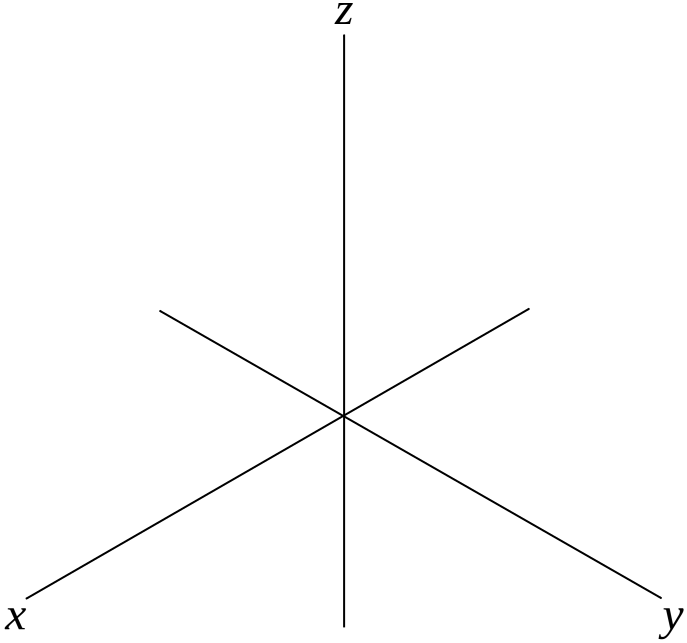
\includegraphics[scale=#1]{3DAxes}\end{center}}
\newcommand{\axespt}[1]{\begin{center}\includegraphics[scale=#1]{3DAxesWithPoint}\end{center}}
\newcommand{\pic}[2]{\begin{center}\includegraphics[scale=#1]{#2}\end{center}}
\newcommand{\comps}[1]{\langle #1_1,#1_2,#1_3\rangle}
\newcommand{\compslong}[3]{\langle #1, #2, #3\rangle}

\begin{document}
	\begin{flushright}
		{\large \textbf{Homework 3}}{\textbf{\scriptsize{/test prep 1}}}\hfill Name: \line(1,0){200}\\
		{\mbox{\hspace{1.75mm}}\small(front and back)}\hfill{\small (please print neatly!)}\mbox{\hspace{0.7in}}
	\end{flushright}
	\vspace{-1.5mm}
	\begin{adjustwidth}{0.5in}{0.5in}
		\begin{tcolorbox}[
			arc=0pt, colback=white, colframe=black, boxrule=0.5pt, before upper={\parindent15pt \parskip=3mm}]
			
			{\noindent\textbf{Directions:} Answer each of the following \textbf{\ul{four} (4)} questions, making sure to read the instructions for \ul{each question} as you proceed. \par
			
			\textbf{Make sure that your submission meets the criteria of the \ul{Homework Policy} on the \texttt{Homework} tab of the course webpage!}
			
			\begin{center}\fbox{\,\textbf{Note:} Questions 1--3 are good quiz prep; all are good exam prep!\,}\end{center}
		
			\hfill\textbf{Due date:} Monday, July 17}
		\end{tcolorbox}
	\end{adjustwidth}
		
	\begin{enumerate}
		\item Solve the initial value problem
		\[y''+4y=x^2e^{-x}-x\sin{x}+4x,\quad y(0)=0,\quad y'(0)=1.\]
		\sol
%		\hint{A good guess for $\text{RHS}=-x\sin{x}$ is 
%		\[(Ax+B)\sin{x}+(Cx+D)\cos{x}\text{\quad(or the equivalent).}\]}
		
		\newpage
		
		\item Write down the general solution for each of the following non-homogeneous ODEs. 
		
		\hint{\ul{Do not} use undetermined coefficients!}
		\begin{enumerate}[itemsep=2in]
			\item $y''+4y'-5y=16e^{x/2}$
			\item $2y''+8y'+8y=2t^{-2}e^{-2t},\quad t>0$
			\item $y''-2y'+y=3\sec(2t),\quad t<\frac{\pi}{6}$
			\item $y''-5y'+6y=g(t)$\quad\hint{$g(t)$ is an arbitrary continuous function.}
		\end{enumerate}
	
		\newpage
		
		\item Show that the functions $y_1$ and $y_2$ satisfy the corresponding homogeneous equation; then, find a particular solution of the given non-homogeneous ODE. Throughout, assume $x>0$.
		\[x^2y''+xy'+(x^2-0.25)y=3x^{3/2}\sin(x);\quad y_1=\frac{\sin{x}}{\sqrt{x}},\quad y_2=\frac{\cos{x}}{\sqrt{x}}\]
		\sol
		
		\newpage
		
		\item Find the Laplace transform for each of the following functions. Throughout, assume that $a$ and $b$ are real constants and that $i=\sqrt{-1}$ is the imaginary unit.
		\begin{enumerate}[itemsep=1.625in]
			\item $f(t)=1$
			\item $f(t)=t^2$
			\item $f(t)=\sin(b t)$\quad\hint{$\sin(bt)=\frac{e^{i b t}-e^{-i b t}}{2i}$}
			\item $f(t)=t^2 e^{a t}$\quad\hint{Use integration by parts!}
			\item $f(t)=5\sin(b t)-2t^2 e^{a t}$
		\end{enumerate}
		
	\end{enumerate}
\end{document}